\documentclass[11pt]{article}
\usepackage[letterpaper,top=2cm,bottom=2cm,left=2cm,right=2cm,marginparwidth=1.75cm]{geometry}

 % Useful packages 
\usepackage{hyperref}
\usepackage{biblatex}
\usepackage{amsfonts}
\usepackage{libertinus}
\usepackage{libertinust1math}


\addbibresource{Bib.bib}
\usepackage{mathtools}
\DeclarePairedDelimiterXPP\BigOSI[2]%
  {\mathcal{O}}{(}{)}{}%
  {\SI{#1}{#2}}
\makeatletter

\DeclareRobustCommand{\dbar}{\text{\addbar@{0.2ex}{0.25em}{1}}d}
\DeclareRobustCommand{\qbar}{\text{\addbar@{-1.25ex}{0.13em}{1}}q}
\DeclareRobustCommand{\pbar}{\text{\addbar@{-1.25ex}{-0.01em}{1}}p}

\newcommand{\addbar@}[3]{%
  \makebox[0pt][l]{%
    \raisebox{#1}[0pt][0pt]{%
      \kern#2
      \scalebox{#3}[0.8]{$\m@th\mathchar"84$}%
    }%
  }%
}

\makeatother


  
\usepackage{braket}
\usepackage{amsmath}
\usepackage{empheq}
\usepackage[most]{tcolorbox}
\usepackage{amsmath}
\usepackage{mathrsfs}
\usepackage[utf8]{inputenc}
\usepackage{graphicx}
\usepackage{float}
\usepackage{parskip}
\usepackage{comment}
\usepackage{mhchem}
 \usepackage{tabularx}
 \usepackage{titling}
  \usepackage[explicit]{titlesec}
\usepackage{fancyhdr}
\setlength{\droptitle}{3em} 

\title{Statistical Physics I}
\author{Thomas Brosnan}
\date{Notes taken in Professor Manuela Kulaxizi's class, Michaelmas Term 2023}


\numberwithin{equation}{section}

\newtcbox{\mymath}[1][]{%
    nobeforeafter, math upper, tcbox raise base,
    enhanced, colframe=blue!30!black,
    colback=blue!30, boxrule=1pt,
    #1}
\newenvironment{bux}
    {
    \empheq[box=\tcbhighmath]{align}
   }{
    \endempheq
    }
    \newenvironment{bux*}
    {
    \empheq[box=\tcbhighmath]{align*}
   }{
    \endempheq
    }
\newenvironment*{nothing}{}{} 
\newcommand{\hsp}{\hspace{8pt}}

\newcommand*{\sectionFont}{%
  \LARGE\bfseries
}

    
\numberwithin{equation}{section}

\makeatletter
\let\Title\@title % Copy the title to a new command
\makeatother

%change this RGB value to change the section background colour 
\definecolor{mycolor1}{RGB}{161, 106, 222}
\colorlet{SectionColour}{mycolor1}
%subsection background colour 
\definecolor{mycolor2}{gray}{0.8}
\colorlet{subSectionColour}{mycolor2}

\definecolor{mycolor3}{RGB}{255,255,255}
\colorlet{subsubSectionColour}{mycolor3}
    
\begin{document}

\maketitle

\newpage
\vspace*{\fill}
%quote 
\begin{center}
    \Large 
   The [second] law that entropy always increases, holds, I think, the supreme position among the laws of Nature. … if your theory is found to be against the second law of thermodynamics I can give you no hope; there is nothing for it but to collapse in deepest humiliation.”

- Sir Arthur Stanley Eddington
\end{center}
\vspace*{\fill}
\newpage
\tableofcontents
    
    

%definition of sections, footers and headers\
\section*{}
% For \section
 \titleformat{\section}[block]{\sectionFont}{}{0pt}{%
 \fcolorbox{black}{SectionColour}{\noindent\begin{minipage}{\dimexpr\textwidth-2\fboxsep-2\fboxrule\relax}\thesection  \hsp #1 {\strut} \end{minipage}}}
% For \subsection
 \titleformat{\subsection}[block]{\bfseries}{}{0pt}{%
 \fcolorbox{black}{subSectionColour}{\noindent\begin{minipage}{\dimexpr\textwidth-2\fboxsep-2\fboxrule\relax}\thesubsection  \hsp #1 {\strut} \end{minipage}}}
% For \section*
 \titleformat{name=\section, numberless}[block]{\sectionFont}{}{0pt}{%
 \fcolorbox{black}{SectionColour}{\noindent\begin{minipage}{\dimexpr\textwidth-2\fboxsep-2\fboxrule\relax} #1 {\strut} \end{minipage}}}
  % For \subsection*
 \titleformat{name=\subsection, numberless}[block]{\bfseries}{}{0pt}{%
 \fcolorbox{black}{subSectionColour}{\noindent\begin{minipage}{\dimexpr\textwidth-2\fboxsep-2\fboxrule\relax} #1 {\strut} \end{minipage}}}
 % For \subsubsection
\titleformat{\subsubsection}[block]{\bfseries}{}{0pt}{%
 \fcolorbox{black}{subsubSectionColour}{\noindent\begin{minipage}{15cm}\thesubsubsection \hsp #1 {\strut} \end{minipage}}}
  % For \subsubsection*
 \titleformat{name=\subsubsection, numberless}[block]{\bfseries}{}{0pt}{%
 \fcolorbox{black}{subsubSectionColour}{\noindent\begin{minipage}{15cm} #1 {\strut} \end{minipage}}}

\newpage
%header 
\pagestyle{fancy}
\fancyhf{} % Clear all header and footer fields
\fancyhead[L]{\Title}
\fancyhead[R]{\nouppercase{\leftmark}}
\fancyfoot[C]{-~\thepage~-}
\renewcommand{\headrulewidth}{1pt}


\normalsize
\newpage
\tcbset{highlight math style={boxsep=5mm,colback=green!0!red!0!blue!0}}

\section{Thermodynamics}

\subsection{System} 
\begin{itemize}
    \item In thermodynamics we usually deal with a macroscopic system, comprising of $N$
constituents, where $1>> \frac{1}{\sqrt{N}}$. The properties of these systems then arise as a result of symmetries and fundamental laws of physics. 
\end{itemize}
 

\subsection{Static states}
\begin{itemize}
     \item Macroscopic variables sense only coarse spatial averages of the coordinates describing the motion of the constituents.   

There are naturally two types of averaging, over time and over distance. These are implicit in macroscopic variables. 
 \end{itemize}

\subsection{Simple systems}
\begin{itemize}
    \item Simple systems are microscopically homogeneous , isotropic, uncharged and large enough so that we need not take into account surface/boundary effects. 
\end{itemize}

\subsection{Thermodynamic parameters}
\begin{itemize}
    \item Volume $V=\sum_{j=1}^mV_j$ for j sub-systems.
    \item $\{ N_i \}$, Chemical composition of the system, $i$ denotes the type of constituent (i.e. different molecules). 
    \item Internal Energy $E$, (or $U$), is the energy contained in the system excluding the center of mass motion and an external energy the system has as a whole due to external forces. 

These parameters are known as extensive parameters (meaning they scale with the system), otherwise they would be known as intensive parameters. 
\end{itemize}

\subsection{Postulate 1}
\begin{itemize}
    \item There exists states called \textbf{equilibrium states} of simple thermodynamic systems, that are completely characterised by the values of $E$, $V$ and $\{ N_1, N_2,...,N_r \}$ for systems comprised of $r$ different species of constituents. 

\end{itemize}

\subsection{Walls and Constraints/ Boundaries}
\begin{itemize}
    \item Walls/Boundaries separate the system from the environment and provide boundary conditions. 
Processes are initiated and the extensive parameters changed by the manipulation of the walls/boundaries. 
\end{itemize}

\subsection{Types of Boundaries}
\begin{itemize}
    \item A wall that is impermeable to the flow of heat is \textbf{adiabatic }, other wise it is \textbf{di-thermal}. 
    \item A wall that does not allow mechanical work is \textbf{mechanically isolated}, (Volume preserved).
    \item A wall that does not allow chemical work is \textbf{chemically isolated}, ($\{N_i\}$ preserved). 

\end{itemize}
\subsection{Postulate 2}
\begin{itemize}
    \item There exists walls, adiabatic, with the property that the work done in taking an adibabatically enclosed system between two given states is determined entirely by the States and is independent of external conditions. 

\end{itemize}
\subsection{Quasi state process}
\begin{itemize}
    \item A quasi state process is a process that preserves the equilibrium of the system through out. 
\end{itemize}
\subsection{1st Law of thermodynamics}
\begin{itemize}
    \item The heat flux to a system in any process that leaves the number of constituents unchanged is simply the difference in the internal energies of the initial and final states.

For simple systems and $N = $ constant during the process, if we define positive work to be work done by the system, then:
\begin{empheq}[box=\tcbhighmath]{equation}
\begin{split}
   \dbar W = PdV
\end{split}
\end{empheq}
Here $P$ is the pressure and $V$ is the volume. The $\dbar$ in the differential is there to note that this is not an exact differential. 

The first law then tells us that:
\begin{empheq}[box=\tcbhighmath]{equation}
\begin{split}
\label{eqn:2.1}
   \dbar Q = dE + \dbar W = dE + PdV - \sum_{i=1}^r\mu_idN_i
\end{split}
\end{empheq}
Here the $\mu_i$ are the different chemical potentials of the constituents $i$.


\end{itemize}

\subsection{Exact differential }
\begin{itemize}
    \item An exact differential of a function $f(a_1,a_2,...,a_n)$ is given by:
\begin{empheq}[box=\tcbhighmath]{equation}
\begin{split}
   df \equiv \sum_{i=1}^n(\frac{\partial f}{\partial a_i})da_i
\end{split}
\end{empheq}
This also means that:
\begin{empheq}[box=\tcbhighmath]{equation}
\begin{split}
   \frac{\partial^2f}{\partial a_i \partial a_j} = \frac{\partial^2f}{\partial a_j \partial a_i}, ~~~\forall ~ i,j
\end{split}
\end{empheq}
Anything of not of this form is inexact and denoted with a $\dbar$

\end{itemize}

\subsection{Basic problem in thermodynamics}
\begin{itemize}
    \item The basic problem in thermodynamics is the determinism of the equilibrium state resulting after the removal of all internal constraints in a closed($\implies$ totally isolated) composite system.

\end{itemize}
\subsection{2nd Law of thermodynamics}
\begin{itemize}
    \item There exists a function $S$ (entropy) of the extensive parameters of any composite system defined for equilibrium states and has the property that it is maximised over the values assumed by the extensive parameters in the absence of internal constraints. 
    \item This function $S(E,V,N)$ is called the fundamental equation or relation. 
\end{itemize}

\subsection{Further restrictions on $S$}
\begin{itemize}
    \item The entropy of any composite system is additive over its subsystems (i.e. $S$ is extensive itself)
    \item Also $S$ is continuous, differentiable and monotonically increasing function of the energy $E$. 
This means that for $r$ subsystems:

\item We can also find that if we scale our system by $\lambda$, then according to the above restrictions: 
\begin{empheq}[box=\tcbhighmath]{equation}
\begin{split}
   S(E,V,N) \rightarrow S(\lambda E, \lambda V, \lambda N) = \lambda S(E,V,N)
\end{split}
\end{empheq}
This makes $S$ a homogeneous degree 1 function.


\end{itemize}
\subsection{Homogeneous degree $k$ function}
\begin{itemize}
    \item A function $f(\lambda x_1,\lambda x_2,...,\lambda x_n) = \lambda^k f(x_1,x_2,...,x_n)$ is said to be homogeneous of degree $k$. 
\end{itemize}
\subsection{3rd Law of thermodynamics } 
\begin{itemize}
\item \begin{empheq}[box=\tcbhighmath]{equation}
\begin{split}
   \frac{\partial E}{\partial S} = 0 \implies S=0 
\end{split}
\end{empheq}
Here the quantity $\frac{\partial E}{\partial S} $ is essentially temperature.
\end{itemize}
\subsection{Intensive parameters}
\begin{itemize}
    \item From the fundamental equation we can theory solve $E=E(S,V,N_1,N_2,...,N_r)$, $E$ then must satisfy:
\begin{empheq}[box=\tcbhighmath]{equation}
\begin{split}
  E(\lambda S,\lambda V,\lambda N_1,\lambda N_2,...,\lambda N_r) = \lambda E(S,V,N_1,N_2,...,N_r)
\end{split}
\end{empheq}
\item Then taking the total derivative:
\begin{empheq}[box=\tcbhighmath]{equation}
\begin{split}
  dE  = \left(\frac{\partial E}{\partial S} \right)dS +\left(\frac{\partial E}{\partial V} \right)dV+\sum_{i=1}^r\left(\frac{\partial E}{\partial N_i} \right)dN_i
\end{split}
\end{empheq}
Then we define the intensive parameters:
\begin{empheq}[box=\tcbhighmath]{equation}
\begin{split}
 T \equiv \left(\frac{\partial E}{\partial S} \right),~~~-P \equiv \left(\frac{\partial E}{\partial V} \right),~~~\mu_i \equiv \left(\frac{\partial E}{\partial N_i} \right)
\end{split}
\end{empheq}
These are intensive as they do not change under re-scaling of the system. Thus they can be consider homogeneous functions of degree 0 and are all functions of $S,V,N$.   Then the total differential can be written as: 
\begin{empheq}[box=\tcbhighmath]{equation}
\begin{split}
  dE  =TdS -PdV+\sum_{i=1}^r\mu_idN_i
\end{split}
\end{empheq}
\item This can be recognised as the first law of thermodynamics where $-PdV$ is the differential of the mechanical work and $\mu_idN_i$ is the differential of the chemical work.  
\end{itemize}

\subsection{Gibbs Duhem relation }
\begin{itemize}
    \item Choosing $\lambda = \frac{1}{N_k}$, then $T \rightarrow T(\frac{E}{N_k},\frac{V}{N_k},\frac{N_1}{N_k},\frac{N_2}{N_k},...,1,...,\frac{N_r}{N_k}) = T(E,V,N_1,N_2,..,N_r)$. Thus we can see the necessary independent parameters are $r+1$ instead of $r+2$. This implies there is a relation between them.

This relation is the Gibbs-Duhem relation and to find this we need to use a property of homogeneous functions. 
\end{itemize}

\subsection{Euler's theorem for homogeneous functions }
\begin{itemize}
    \item If $f(\lambda x_1, \lambda x_2, ...,\lambda x_n) = \lambda^k f(x_1,x_2,...,x_n)$, then:
\begin{empheq}[box=\tcbhighmath]{equation}
\begin{split}
 kf(x_1,x_2,...,x_n) = \sum_{i=1}^n \left(\frac{\partial f}{\partial x_i}\right) x_i
\end{split}
\end{empheq}
\item Applying this theorem:
\begin{empheq}[box=\tcbhighmath]{equation}
\begin{split}
  E(S,V,N_1,N_2,...,N_r) = \left( \frac{\partial E}{\partial S}\right)S+\left( \frac{\partial E}{\partial V}\right)V+\sum_{i=1}^r\left( \frac{\partial E}{\partial N_i}\right )N_i 
\end{split}
\end{empheq} 
\item Thus:
\begin{empheq}[box=\tcbhighmath]{equation}
\begin{split}
\label{eqn:1.13}
 E = TS -PV + \sum_{i=1}^r\mu_iN_i
\end{split}
\end{empheq}
\end{itemize}
\subsection{Solving the Gibbs-Duhem relation}
\begin{itemize}
    \item To do this we take the total differential of the above equation and see:
\begin{empheq}[box=\tcbhighmath]{equation}
\begin{split}
   dE = TdS + SdT -PdV -VdP + \sum_{i}\mu dN_i + \sum_iN_id\mu_i
\end{split}
\end{empheq}
But by the first law this must be equal to \ref{eqn:2.1}. Thus we get:
\begin{empheq}[box=\tcbhighmath]{equation}
\label{1.15}
\begin{split}
   SdT -VdP + \sum_iN_id\mu_i =0
\end{split}
\end{empheq}
\item This is our Gibb's-Duham relation.
\end{itemize}
\subsection{Thermodynamic configuration space}
\begin{itemize}
    \item We define a thermodynamic configuration space.

For a simple system such a space is spanned by co-ordinate axes that correspond to $S,E,V,N_1,N_2,...,N_r$.  Then $S(E,V,N_1,N_2,...,N_r)$ defines a surface in this space that conforms to various requirements that $S$ itself satisfies.  

Any system will proceed from a state $A$ (point $A$ on the surface of $S$) to state $B$, iff $S$ is maximised at $B$ compared to all other states. 

If we have $S_a <  S_b$ then the process has a unique direction from lower to higher entropy and is irreversible. 

It is possible for the process to be reversible if $\Delta S =0$. 

\end{itemize}

\subsection{Fundamental relation}
\begin{itemize}
    \item We can consider either $E(S,V,N_i)$ or $S(E,V,N_i)$ to be fundamental relations. But we cannot however, consider $E(T,V,N_i)$ or $S(T,V,N_i)$ to be fundamental as by the definition of $T$ we must take a derivative and there we know we loose information relating to what is held constant. 
\end{itemize}


\subsection{Free expansion}
\begin{itemize}
    \item If a system changes by free expansion this means that $\dbar W =0$ through out this process.
\end{itemize}

\subsection{Thermodynamic Potentials}
\begin{itemize}
    \item We can construct functions of intensive parameters that give as much information as $S$ and $E$, i.e. they are fundamental relations.  These potentials are Legendre transforms of either $E(S,V,N_i)$ or $S(E,V,N_i)$. Through examining their differentials one can find many partial derivative relations. These potentials are extensive functions. Just as in mechanics, the system will tend towards a lower value of a potential and at equilibrium, under the constraints as listed below, the potential will take the unchanging minimum value.
\subsubsection{Helmholtz Free} 
\begin{itemize}
    \item This is $\mathcal{F}(T,V,N_i)$ and is given by:
\begin{empheq}[box=\tcbhighmath]{equation}
\begin{split}
 \mathcal{F} = E-TS
\end{split}
\end{empheq}
We use $\mathcal{F}$ in the case of an isothermal process along with there being chemical and mechanical isolation. $\mathcal{F}$ also has:
\begin{empheq}[box=\tcbhighmath]{equation}
\begin{split}
 - P = \left(\frac{\partial F}{\partial V}\right),~~~ - S = \left(\frac{\partial F}{\partial T}\right),~~~ \mu_i = \left(\frac{\partial F}{\partial N_i}\right)
\end{split}
\end{empheq}

\end{itemize}
\subsubsection{Gibbs free}
\begin{itemize}
    \item This is $\mathcal{G}(T,P,N_i)$ and is given by:
\begin{empheq}[box=\tcbhighmath]{equation}
\begin{split}
  \mathcal{G} = F+PV
\end{split}
\end{empheq}
We use $\mathcal{G}$ in the case of an isothermal and Isobaric system along with chemical and mechanical isolation.  $\mathcal{G}$ also has:
\begin{empheq}[box=\tcbhighmath]{equation}
\begin{split}
  V = \left(\frac{\partial G}{\partial P}\right),~~~ - S = \left(\frac{\partial G}{\partial T}\right),~~~ N_i = \left(\frac{\partial G}{\partial \mu_i}\right)
\end{split}
\end{empheq}
\end{itemize}
\subsubsection{Grand canonical potential}
\begin{itemize}
    \item This is $\mathcal{J}(T,V,\mu_i)$ and is given by:
\begin{empheq}[box=\tcbhighmath]{equation}
\begin{split}
   \mathcal{J} = E -TS - \sum_i\mu_iN_i
\end{split}
\end{empheq}
We use $\mathcal{J}$ in the case of an isothermal process and fixed chemical potential, along with mechanical isolation. $\mathcal{J}$ also has:
\begin{empheq}[box=\tcbhighmath]{equation}
\begin{split}
  P =- \left(\frac{\partial \mathcal{J}}{\partial V}\right),~~~  S = -\left(\frac{\partial \mathcal{J}}{\partial T}\right),~~~ N_i = -\left(\frac{\partial \mathcal{J}}{\partial \mu_i}\right)
\end{split}
\end{empheq}
\item We can also see that applying \ref{eqn:1.13} to the grand canonical potential leads to:
\begin{bux}
    \begin{split}
        \mathcal{J} = -PV
    \end{split}
\end{bux}
\end{itemize}
\subsubsection{Enthalpy}
\begin{itemize}
    \item This is $\mathcal{H}(S,P,N_i)$ and is given by:
\begin{empheq}[box=\tcbhighmath]{equation}
\begin{split}
\mathcal{H} = E + PV
\end{split}
\end{empheq}
We use $\mathcal{H}$ in the case of an Isobaric process along with thermal and chemical isolation.  $\mathcal{H}$ also has:
\begin{empheq}[box=\tcbhighmath]{equation}
\begin{split}
  P = \left(\frac{\partial H}{\partial V}\right),~~~  S = \left(\frac{\partial H}{\partial T}\right),~~~ \mu_i = \left(\frac{\partial H}{\partial N_i}\right)
\end{split}
\end{empheq}
\end{itemize}
\end{itemize}

\subsection{Maxwell's relations}
\begin{itemize}
    \item In examining the different potentials above, one can use the fact that they are exact to derive extra partial derivative relations between the parameters. These relations come from the fact that it does not matter which order you take the derivatives. i.e. $\frac{\partial^2E}{\partial V \partial S} = \frac{\partial^2E}{\partial S \partial V}$. The relations discovered are:
\begin{empheq}[box=\tcbhighmath]{equation}
\begin{split}
 \left(\frac{\partial T}{\partial V}\right)_{S} = -\left(\frac{\partial P}{\partial S}\right)_V,~~~\left(\frac{\partial T}{\partial P}\right)_S = \left(\frac{\partial V}{\partial S}\right)_P \\ \left(\frac{\partial V}{\partial T}\right)_P = - \left(\frac{\partial S}{\partial P}\right)_T,~~~\left(\frac{\partial P}{\partial T}\right)_V = \left(\frac{\partial S}{\partial V}\right)_T
\end{split}
\end{empheq}
\item However it should be noted that if one comes to a problem where you can write down one of the thermodynamic potentials and solve the problem, then you will not need to use any of the Maxwell's relations through out that problem, provided the correct potential is chosen. 
\end{itemize}

\subsection{Concavity/Convexity}
\begin{itemize}
    \item A function $f(x_1,x_2,...,x_n)$ with a parameter $t \in [0,1]$, is concave iff:
\begin{empheq}[box=\tcbhighmath]{equation}
\begin{split}
 f(tx_1+(1-t)y_1,...,tx_n+(1-t)y_n) \geq tf(x_1,...,x_n)+(1-t)f(y_1,...,y_n)
\end{split}
\end{empheq}
\item $f$ is instead convex iff:
\begin{empheq}[box=\tcbhighmath]{equation}
\begin{split}
 f(tx_1+(1-t)y_1,...,tx_n+(1-t)y_n) \leq tf(x_1,...,x_n)+(1-t)f(y_1,...,y_n)
\end{split}
\end{empheq}
Concavity means all tangent lines are above the graph of the function, where as convexity means all tangent lines are below the graph of the function. 

 \item  For fixed $N$ the thermodynamic potentials defined by the Legendre transform of $E(S,V,N_i)$ and $S(E,V,N_i)$ are convex functions of there extensive variables and concave functions of their intensive variables.

\end{itemize}

\subsection{Hessian matrix}
\begin{itemize}
    \item For functions $f: \mathbb{R}^n \rightarrow \mathbb{R}$ of many variables which are at least twice differentiable the hessian matrix is defined as:
\begin{empheq}[box=\tcbhighmath]{equation}
\begin{split}
 H =  \begin{pmatrix}
       \frac{\partial^2 f}{\partial x_1^2} &\cdot & \cdot & \cdot & \frac{\partial^2 f}{\partial x_1 \partial x_n} \\
       \cdot&\cdot&~&~& \cdot  \\
       \cdot&~&~\cdot&~& \cdot \\
       \cdot&~&~&\cdot~& \cdot \\
       \frac{\partial^2 f}{\partial x_m\partial x_1} &\cdot & \cdot & \cdot & \frac{\partial^2 f}{\partial x_1 \partial x_m}
    \end{pmatrix}
\end{split}
\end{empheq}
Then if the hessian matrix evaluated at a point $H(x_1^0,x_2^0,...,x_n^0)$, is positive definite then it has positive eigenvalues and thus there is a local minimum at $\textbf{x}_0$. Likewise if $H(x_1^0,x_2^0,...,x_n^0)$ is negative definite there is a max at $\textbf{x}_0$. If there are both positive and negative eigenvalues then $\textbf{x}_0$ is a saddle point otherwise if $det(H)=0$, then the test is inconclusive. 

\item For functions $f(x_1,x_2)$, twice differentiable, $f$ is concave iff:
\begin{empheq}[box=\tcbhighmath]{equation}
\begin{split}
 \frac{\partial^2f}{\partial x_i^2}\leq0,~i=1,2,~~\text{and} ~ \frac{\partial^2f}{\partial x_1^2}\frac{\partial^2f}{\partial x_2^2}-\frac{\partial^2f}{\partial x_1 \partial x_2} \geq0
\end{split}
\end{empheq}
And $f$ is convex iff:
\begin{empheq}[box=\tcbhighmath]{equation}
\begin{split}
 \frac{\partial^2f}{\partial x_i^2}\geq0,~i=1,2,~~\text{and} ~ \frac{\partial^2f}{\partial x_1^2}\frac{\partial^2f}{\partial x_2^2}-\frac{\partial^2f}{\partial x_1 \partial x_2} \geq 0
\end{split}
\end{empheq}



\end{itemize}

\subsection{Physical properties }
\begin{itemize}
    \item These are measurable properties of materials defined through the thermodynamic variables. 
\subsubsection{Heat Capacities }
\begin{itemize}
    \item There is the heat capacity at constant volume $C_V$:
\begin{empheq}[box=\tcbhighmath]{equation}
\begin{split}
 C_V \equiv \left( \frac{d Q}{dT}\right)_V = \left( \frac{\partial E}{\partial T}\right)_{V,N}
\end{split}
\end{empheq}
\item And the heat capacity at constant pressure $C_P$:
\begin{empheq}[box=\tcbhighmath]{equation}
\begin{split}
C_P \equiv \left( \frac{d Q}{dT}\right)_P = \left( \frac{\partial E}{\partial T}\right)_{P,N}+P\left( \frac{\partial V}{\partial T}\right)_{P,N} = \left( \frac{\partial H}{\partial T}\right)_{P,N}
\end{split}
\end{empheq}

\end{itemize}
\subsubsection{Coefficient of thermal expansion }
\begin{itemize}
    \item This is $\alpha$ defined as:
\begin{empheq}[box=\tcbhighmath]{equation}
\begin{split}
\alpha \equiv  \frac{1}{V}\left( \frac{\partial V}{\partial T}\right)_{P,N}
\end{split}
\end{empheq}


\end{itemize}
\subsubsection{Coefficient of isothermal/isentropic  compressability}
\begin{itemize}
    \item The coefficient of isothermal compressability is given by:
\begin{empheq}[box=\tcbhighmath]{equation}
\begin{split}
\kappa_T \equiv -\frac{1}{V} \left( \frac{\partial V}{\partial P}\right)_{T,N}
\end{split}
\end{empheq}
\item And the coefficient of isentropic (though really here we mean adiabatic plus reversible but we assume everything is quasistatic so we can just say isentropic) compressability is:
\begin{empheq}[box=\tcbhighmath]{equation}
\begin{split}
\kappa_s \equiv -\frac{1}{V} \left( \frac{\partial V}{\partial P}\right)_{S,N}
\end{split}
\end{empheq}
\end{itemize}
\item From these definitions the following properties can be shown:
\begin{bux}
\begin{split}
\label{eqn:1.35}
      &  C_P - C_V = TV\frac{\alpha^2}{\kappa_T} \\
       & \frac{C_P}{C_V} = \frac{\kappa_T}{\kappa_S} \\
          C_V  = TV& \frac{\alpha^2 \kappa_S}{\kappa_T(\kappa_T - \kappa_S)},~~~C_P = TV\frac{\alpha}{\kappa_T- \kappa_S}
\end{split}
\end{bux}
\end{itemize}

\subsection{Consequences of stability }
\begin{itemize}
    \item Due to convexity $\frac{\partial^2 S}{\partial E^2} < 0 $, but $\frac{\partial S}{\partial E} = \frac{1}{T} $, This implies that:
\begin{bux}
\begin{split}
      \frac{1}{T^2}&\left(\frac{\partial T}{\partial E} \right)  = - \frac{1}{T^2C_V} <0 \\
&\implies C_V>0
\end{split}
\end{bux}
Then we can use relations \ref{eqn:1.35} to get that $C_P > C_V > 0$.


Similarly, $\frac{\partial^2 F}{\partial V^2} >0 $ implies that:
\begin{bux}
    \begin{split}
         \kappa_S > 0
    \end{split}
\end{bux}
And then once again by relations \ref{eqn:1.35}, $\kappa_T> \kappa_S > 0$. 


\end{itemize}

\subsection{Phase transitions }
\begin{itemize}
    \item A phase is a state of matter with uniform properties such that at thermodynamic equilibrium a characteristic state equation for the state exists. 

We will consider phase transitions as the failure of equilibrium/stability conditions .

There are two large classes of phase transitions.
\end{itemize}    

\subsection{First order phase transitions} 
\begin{itemize}
    \item Also known as discontinuous, here the different phases are at different regions in the thermodynamic configuration space.  In these transitions the derivative of the thermodynamic potential describing the system is not continuous. 
\end{itemize}

\subsection{Second order phase transition} 
\begin{itemize}
    \item Also known as continuous phase transition, here the two phases are continuous in the thermodynamic equilibrium space. 

\end{itemize}


\subsection{Clausius-Clapeyron equation}
\begin{itemize}
\item At a first order transition the Gibbs free energy at the point of transition is $\mathcal{G} = \mathcal{G}^{(1)} + \mathcal{G}^{(2)}$, where $\mathcal{G}^{(1)}$ and $\mathcal{G}^{(2)}$, are the Gibbs free energy of phase $1$ and $2$, respectively. Then we have that
\begin{bux}
\begin{split}
    \left( \frac{\partial G}{\partial T}\right) = - S_{(1)} \neq S_{(2)} \\ 
\left( \frac{\partial G}{\partial P}\right) = - V_{(1)} \neq V_{(2)}
\end{split}
\end{bux}

For a first order phase transition the pressure remains the same while the volume increases from $V \rightarrow V'$ because the two phases have different densities.  

At the boundary where phases coexist, so $d\mathcal{G} =0_{tot}$, this is due to the fact that $\mathcal{G}$ wants to be at a minima at equilibrium for the conditions of constant pressure and temperature. So if  $T$ and $V$ are fixed as we cross the phase boundary then  we get that:
\begin{bux}
    \begin{split}
        d\mathcal{G}_{tot} = 0 = \mu_1dN_1 + \mu_2dN_2
    \end{split}
\end{bux}
But since we are dealing with an isolated system $dN_1 = -dN_2$. Here $N_i$ is the number of particles in phase $i$.  These two equations tell us that $\mu_1 = \mu_2$. Also here we can use the Gibbs Duhem relation \ref{1.15},  to use the fact that $\mu_1 = \mu_2$ to write down:
\begin{bux}
\begin{split}
   & -\frac{S_1}{N_1}dT + \frac{V_1}{N_1}dP = -\frac{S_2}{N_2}dT + \frac{V_2}{N_2}dP  \\ 
& \implies dP(\frac{V_1}{N_1} - \frac{V_2}{N_2}) = dT(\frac{S_1}{N_1} - \frac{S_2}{N_2}) \\
& \implies \frac{dP}{dT}\bigg\rvert_{across~boundary} = \frac{\Delta s}{\Delta v}
\end{split}
\end{bux}
Where the final term is in terms of specific volume $v$ and entropy $s$. If we then define the latent heat per particle as $l \equiv T\Delta S$, which we can consider constant as this phase change we are discussing is at constant temperature. Thus the  Clausius–Clapeyron equation is:
\begin{bux}
    \begin{split}
         \frac{dP}{dT}= \frac{l}{T\Delta v}
    \end{split}
\end{bux}
This latent heat is always specified with a name that tells you which phase transition it is from and to, eg. the latent heat of vaporisation,sublimation, etc...
There is no latent heat in second order phase transitions.
\end{itemize}

\subsection{Gibbs phase rule }
\begin{itemize}
    \item This gives us an expression for the number of thermodynamic degrees of freedom, If a system can exist in $M$ possible phases and has $r$ constituents, this means we have $2+M(r-1)$ independent variables. The $2$ comes from temperature and pressure and the $M(r-1)$ comes from the $r$ constituents, which have a Gibbs-Duhem relationship for each phase. Then if the phases of each constituent are in equilibrium with each other we must have that 
$\forall~i=1,2,...,r,~~ \mu_i^{(1)}=\mu_i^{(2)}=...=\mu_i^{(M)}$. Thus there are an extra $r(M-1)$ equations. Thus the total number of degrees of freedom are $f =2+M(r-1)-r(M-1) $, thus:
\begin{bux}
    \begin{split}
        f  = r+2-M
    \end{split}
\end{bux}
\end{itemize}

\subsection{Critical point of transition}
\begin{itemize}
    \item If we have a region in the phase space where $\frac{\partial P}{\partial V}>0$, the this implies that $\kappa_T<0$, which is a violation of stability. So phase transition must take place at the point where this begins to happen and where there is a point of inflection so that convex shape of the graph also changes to concave at this point too. So:
\begin{bux}
    \begin{split}
        \frac{\partial P}{\partial V} = \frac{\partial^2 P}{\partial V^2} = 0 
    \end{split}
\end{bux}

\end{itemize}
This idea I think is best motivated from the below figure taken from \href{https://bawar.net/data0/books/5d5fe4eb6bdbb/pdf/8_044-Concepts_in_Thermal_Physics-Blundell.pdf}{Concepts in thermal physics by Blundell and Blundell}. 

\begin{figure}[H]
\centering
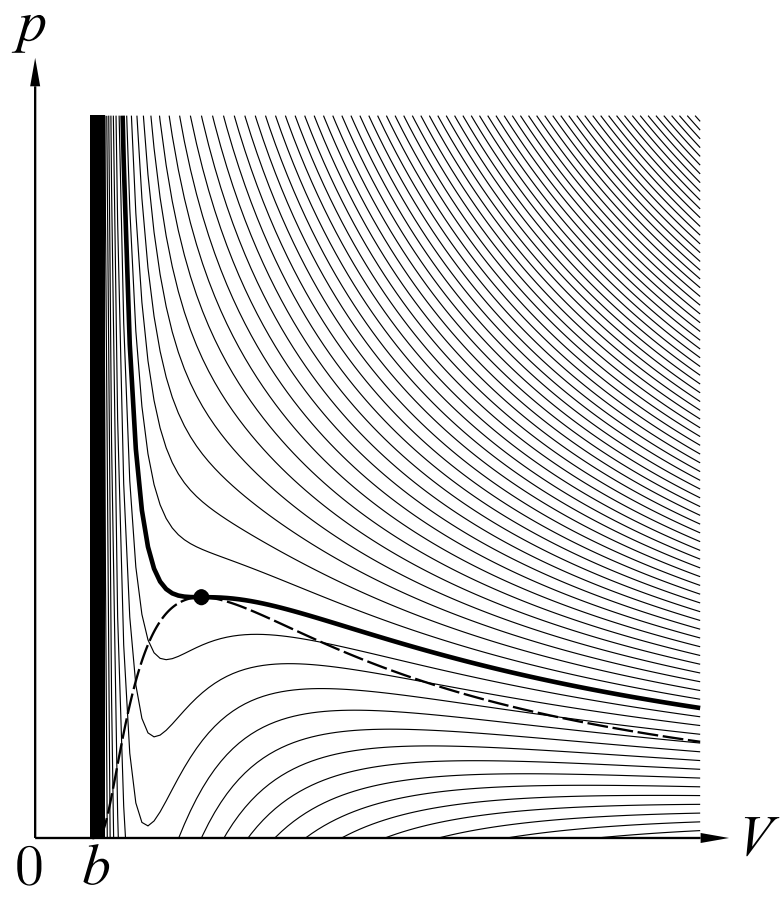
\includegraphics[width=0.8\textwidth]{image.png}
\caption{\label{fig:2}\small \emph{Isotherms of the van der Waals gas. Isotherms towards to the top right of the graph correspond to higher temperatures. The dashed line shows the region in which liquid and vapour are in equilibrium. The thick line is the critical isotherm and the dot marks the critical point. }}
\end{figure}


\newpage

\section{Mathematics of Statistical mechanics}
\subsection{Gamma function}
\begin{itemize}
    \item The Gamma function is the generalisation of the factorial function to non integers ($\Gamma(n+1) = n!$ if $n$ is an integer). It is expressed in the form of an integral and many problems reduce to turning an integral into the gamma function. It is defined as follows: 
\begin{bux}
    \begin{split}
        \Gamma(z) = \int_0^{\infty}t^{z-1}e^{-t}dt
    \end{split}
\end{bux}
Also has the usefull property that $\Gamma(z+1)=z\Gamma(z)$.
\end{itemize}

\subsection{Many variable Gaussian integral}
\begin{itemize}
    \item The Gaussian integral is well known, $\int_{-\infty}^{\infty}e^{-x^2}dx=\sqrt{\pi}$. This can then be generalised to have any sort of multi-variable quadratic powers. If we have have $n$ variables, $x_1,x_2,...,x_n$, then any quadratic combination of these can be written as: 
\begin{bux}
    \begin{split}
        a_{11}x_1^2+a_{12}x_1x_2 + ... = \sum_{i,j=1}^nx_iA_{ij}x_j = \textbf{x}^{T}A\textbf{x}
    \end{split}
\end{bux}
Where here we have introduced the symmetric matrix $A^T=A$ to account for the coefficients $a_{ij}$.  We can use this generalisation via the means of eigenvalues to prove the following integral:
\begin{bux}
    \begin{split}
       \int_{-\infty}^{\infty}dx_1dx_2...dx_ne^{-\frac{1}{2}\textbf{x}^{T}A\textbf{x}} = \frac{(2\pi)^{\frac{n}{2}}}{\sqrt{det(A)}}
    \end{split}
\end{bux}
\item And if we add any linear term:
\begin{bux}
    \begin{split}
       \int_{-\infty}^{\infty}dx_1dx_2...dx_ne^{-\frac{1}{2}\textbf{x}^{T}A\textbf{x}+B^T\textbf{x}} = \frac{(2\pi)^{\frac{n}{2}}}{\sqrt{det(A)}}e^{\frac{1}{2}B^TA^{-1}B}
    \end{split}
\end{bux}

\end{itemize}
\subsection{Beta Function}
\begin{itemize}
    \item Has an integral definition that can be manipulated to be expressed in terms of gamma functions: 
\begin{bux}
    \begin{split}
        B(m,n) = \int_0^{1}x^{m-1}(1-x^{n-1})dx = \frac{\Gamma(m)\Gamma(n)}{\Gamma(m+n)}
    \end{split}
\end{bux}
\end{itemize}
\subsection{Sterling's approximation}
\begin{itemize}
    \item   This approximation is said to only work for large $N$, but has an error of less than 1\% for $N>100$ so its pretty good, this comes from \href{http://hyperphysics.phy-astr.gsu.edu/hbase/Math/stirling.html}{Hyper physics}. See also the graph below as visual proof. The approximation is as follows: 
\begin{bux}
    \begin{split}
        \ln(N!) = \sum_{k=1}^Nln(k) \approx \int_1^Nln(k)dk =  N\ln(N) -N
    \end{split}
\end{bux}
This can be extended to the gamma function:
\begin{bux}
    \begin{split}
         \ln(\Gamma(N+1)) \approx N\ln(N) -N
    \end{split}
\end{bux}
\item This approximation is could be slightly better if instead $  \ln(N!) \approx N\ln(N) -N +\frac{1}{2}\ln(2 \pi N)$. Both of these are shown below. 
\end{itemize}


\begin{figure}[H]
\minipage{0.5\textwidth}
  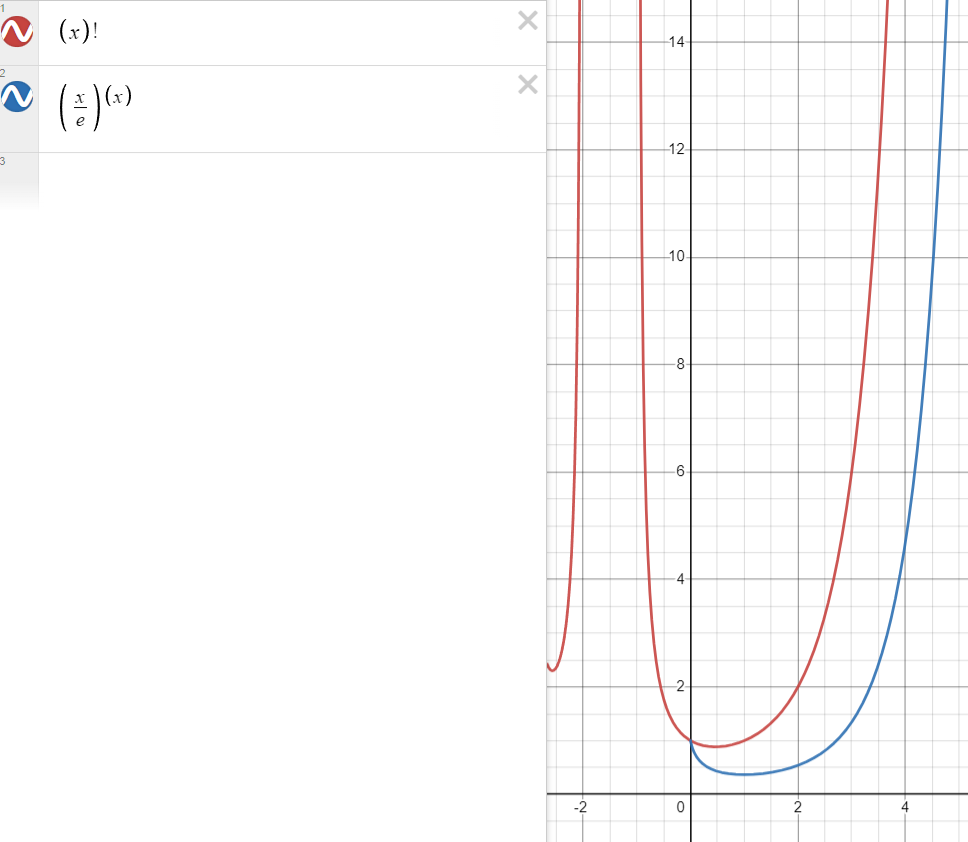
\includegraphics[width=.9\linewidth]{image3.png}
  \caption{Sterling approximation vs $\Gamma(x-1)$ }\label{fig:13}
\endminipage\hfill
\minipage{0.5\textwidth}
  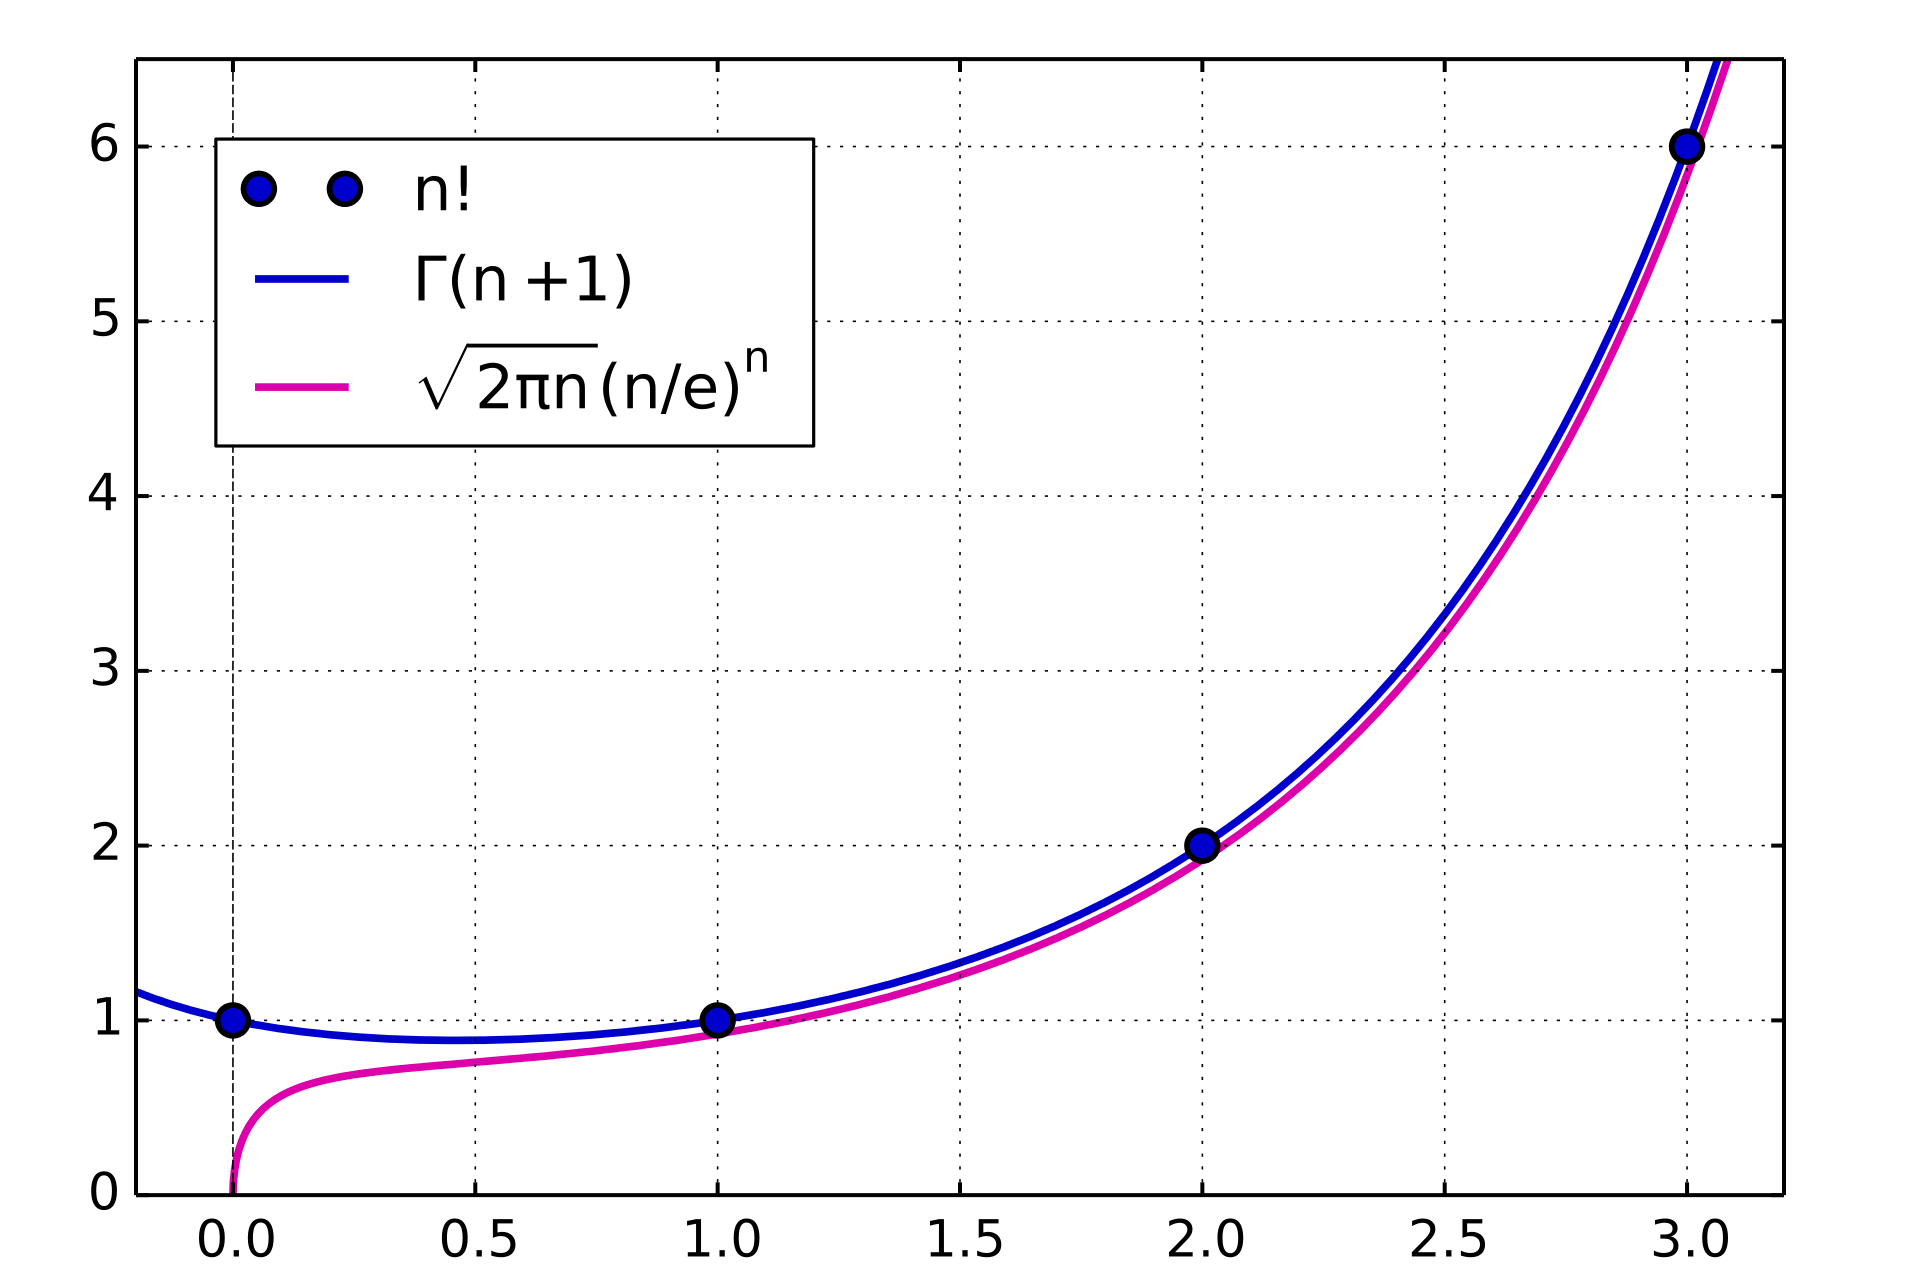
\includegraphics[width=0.9\linewidth]{image2.png}
  \caption{Slightly better Sterling approximation vs $\Gamma(x-1)$}\label{fig:14}
\endminipage\hfill
\end{figure}
\subsection{Area of a Hyper-sphere}
\begin{itemize}
    \item We denote $S^{n-1}(R)$ as the $n-1$ sphere of radius $R$, That is the following set of points:
\begin{bux}
    \begin{split}
      S^{n-1}(R) =  \left\{x\in \mathbb{R}^n \vert~ \sum_{i=1}^n x_i^2  = R^2 \right\}
    \end{split}
\end{bux}
Then we denote $S_{n-1}(R)$ the area of this sphere.  The formula for this can be motivated by considering how one would extend spherical co-ordinates to higher dimensions. For $n-1$ dimensions the co-ordinates would extend as follows

\begin{table}[H]
    \centering
    \begin{tabular}{|c|c|} \hline 
         Cartesian& Spherical\\ \hline 
         $x_1$& $r \cos\phi_1$\\ \hline 
         $x_2$& $r \sin\phi_1\cos\phi_2$\\ \hline 
         $x_3$& $r \sin\phi_1\sin\phi_2\cos\phi_3$\\ \hline 
 .&.\\ \hline 
 .&.\\ \hline 
 .&.\\ \hline 
         $x_{n-2}$& $r \sin\phi_1\sin\phi_2...\sin\phi_{n-2}\cos\phi_{n-1}$\\ \hline 
         $x_{n-1}$& $r \sin\phi_1\sin\phi_2...\sin\phi_{n-2}\sin\phi_{n-1}$\\ \hline
    \end{tabular}
    \caption{Extension of spherical co-ords to $n-1$ dimensions}
    \label{tab:my_label}
\end{table}
Where here $\phi_1 , \phi_2 , ...,\phi_{n-1} \in [0,\pi]$ and $\phi_{n-1} \in [0,2\pi]$.  One can then see that the Jacobian, i.e. the determinant of the Jacobian matrix when changing from $n-1$ Cartesian co-ords to $n-1$ spherical is as follows: 
\begin{bux}
    \begin{split}
       & J = r^{n-1}\sin^{n-2}\phi_1\sin^{n-3}\phi_2...\sin\phi_{n-2} \\ 
\implies dx_1d&x_2...dx_{n-1} =  r^{n-1} d\Omega_{n-1}dr =r^{n-1} dS_{n-1}(1)dr 
    \end{split}
\end{bux}
The last step here is given as the definition of $\Omega_{n}$ is $\Omega_{n} = S_{n-1}/r^{n-1} \implies d\Omega_{n-1}=dS_{n-1}(1)$. Finally to find the area, we consider the following integral two which we know the result: 
\begin{bux}
    \begin{split}
        I_n = \int_{-\infty}^{\infty}\prod_{i=1}^ndx_ie^{-x_i^2} = \pi^{\frac{n}{2}}  
    \end{split}
\end{bux}
And converting to spherical co-ords:
\begin{bux}
    \begin{split}
        &I_n = \int_0^{\infty}r^{n-1}dS_{n-1}(1)dre^{-r^2} , ~~~u=r^2 \\ 
& \implies I_n = \frac{1}{2}S_{n-1}(1) \int_0^{\infty}u^{\frac{n}{2}-1} e^{-u}du = \frac{1}{2}\Gamma(\frac{n}{2}) S_{n-1}(1)
    \end{split}
\end{bux}
Re-arranging: 
\begin{bux}
    \begin{split}
       & S_{n-1}(1)  = \frac{2\pi^{\frac{n}{2}}}{\Gamma(\frac{n}{2})} \\ 
\implies &S_{n-1}(R)  = \frac{2\pi^{\frac{n}{2}}}{\Gamma(\frac{n}{2})}R^{n-1}
    \end{split}
\end{bux}
Where the last jump is from dimensional analysis. 
\end{itemize}

\subsection{Volume of an n-ball}
\begin{itemize}
    \item An $n$-ball is denoted $V^n(R)$ and the volume of this ball $V_n(R)$.  The value of this can be found from considering: 
\begin{bux}
    \begin{split}
    \label{eqn:2.12}        V_n(R) = &\int_{constraints} \prod_{i=1}^ndx_i = \int_0^{R}r^{n-1} dr \int dS_{n-1}  \\ 
&\implies V_n(R)  = \frac{2\pi^{\frac{n}{2}}}{n\Gamma(\frac{n}{2})}R^{n}
    \end{split}
\end{bux}
\end{itemize}

\newpage 

\section{Probability and statistics} 
\subsection{Sample space }
\begin{itemize}
    \item Space of all possible outcomes of an experiment or observed random phenomena. 
\end{itemize}

\subsection{Probability}
\begin{itemize}
    \item If we perform the experiment $N$ times and obtain $n$ positive results, then the probability of a positive result is: 
\begin{bux}
    \begin{split}
        Pr = \lim_{N\rightarrow \infty} \frac{n}{N} 
    \end{split}
\end{bux}
\end{itemize}
\subsection{Random variable}
\begin{itemize}
    \item A function which takes real values and is defined on the sample space. 
\end{itemize}
\subsection{Probability distribution}
\begin{itemize}
    \item Describes the relationship between the random variables and the probabilities that the random variable $X$ will obtain a certain value.   
\end{itemize}
\subsection{Discrete variables }
\begin{itemize}
    \item If the possible values of a random variable are discrete, i.e. $X \in \{ x_1,x_2,...,x_n\}$, then: 
\begin{bux}
    \begin{split}
        Pr[X=x_i] = P_i, ~~~~\sum_{i=1}^nP_i = 1
    \end{split}
\end{bux}
\end{itemize}

\subsection{Continuous variables} 
\begin{itemize}
    \item If the random variable takes on continuous values, i.e. $X \in [a,b] \in \mathbb{R}$, then:
\begin{bux}
    \begin{split}
        Pr[x \leq X \leq x+dx] = \rho(x)dx,~~~~\int_a^b\rho(x)dx =1
    \end{split}
\end{bux}
Here $\rho(x)$ is a probability distribution/density.
\end{itemize}

\subsection{Mean and variance}
\begin{itemize}
    \item The mean $\mu$ is the same as the expectation value of the random variable $\braket{X}$. This takes the following form for the discrete case: 
\begin{bux}
    \begin{split}
        \mu = \braket{X} \equiv \sum_{i=1}^nP_ix_i
    \end{split}
\end{bux}
And in the continuous case: 
\begin{bux}
    \begin{split}
         \mu = \braket{X} \equiv \int_a^b\rho(x)xdx
    \end{split}
\end{bux}
Providing both of these are convergent. 
\item In both cases the variance is defined as $\sigma^2 \equiv \braket{X^2}-\braket{X}^2  $. 

\end{itemize}

\subsection{Common distributions}
\subsubsection{Binomial distribution}
\begin{itemize}
    \item Here there are two outcomes $B$ and $W$ with probabilities $p$ and $q=1-p$. Suppose in $N$ trials we observe $n$ times $B$ and $N-n$ times $W$. To compute the probability in $N$ independent trials to observe $n$ positive results is: 
\begin{bux}
    \begin{split}
        Pr(N,n,p) = \binom Nn p^n(1-p)^{N-n},~~~ \binom Nn = \frac{N!}{n!(N-n)!}
    \end{split}
\end{bux}
This prefactor can be motivated from the following. The number of ways to arrange $n$ distinct objects in $N$ distinct boxes, with $N>n$, is $N(N-1)...(N-n+1) = \frac{N!}{(M-n)!}$.  This just comes from the fact that there are $N$ boxes to put the first object in, $N-1$ to put the second in... repeated until there are no more objects left to place. Then seeing as all the $n$ objects are identical we have to divide by $n!$ to avoid over counting.  leaving us with the above prefactor. 

\item For this distribution $\mu = Np$ and $\sigma = Np(1-p)$. 
\end{itemize}  

\subsubsection{Multinomial distribution}
\begin{itemize}
    \item Generalisation of binomial, for when there are $k$ possible outcomes, with $k>2$ and so $P_i$, $i=1,2,...,k$. Then we we can write: 
\begin{bux}
    \begin{split}
        Pr[X_1=n_1,X_2=n_2,...,X_k=n_k,] = \frac{N!}{n_1!n_2!...n_k!}P_1^{n_1}P_2^{n_2}...P_k^{n_k}
    \end{split}
\end{bux}
Where the total number of trials is $\sum_{i=1}^kn_i =N$.  As well as $\sum_{i=1}^kP_i=1$. 
\end{itemize}

\subsubsection{Poisson distribution}
\begin{itemize}
    \item This distribution that gives us the probability of $k$ events to occur in a fixed time or space interval given that we know that these events occur at a constant rate $r$ in a fixed time interval $t$: 
\begin{bux}
    \begin{split}
        Pr[X=k] = e^{-rt}\frac{(rt)^k}{k!}
    \end{split}
\end{bux}
Or if we know that the average number of events in this given interval is $\lambda$:
\begin{bux}
    \begin{split}
        Pr[X=k] = e^{-\lambda}\frac{\lambda^k}{k!}
    \end{split}
\end{bux}
\item For this distribution both $\mu = \sigma = \lambda$. 
\end{itemize}

\subsubsection{Gaussian distribution}
\begin{itemize}
    \item Is the most common important continuous distribution. Applies to most random phenomena with given average $\mu$ and standard deviation $\sigma$. The distribution takes the form: 
\begin{bux}
    \begin{split}
        \rho(x) = \frac{1}{\sqrt{2\pi \sigma}}e^{-\frac{(x-\mu)^2}{2\sigma^2}}
    \end{split}
\end{bux}
\end{itemize}


\subsection{Central limit theorem }
\begin{itemize}
    \item Suppose that $X_i$, $i=1,2,...,N$ are random independent variables with the same probability distribution $\rho(x)$. If we define a new random variable $Y = X_1+X_2+...+X_N$, then in the limit as $N\rightarrow \infty$ (In practise we have $N>>1$). Then the probability distribution $Pr[y \leq Y \leq y+dy] = \rho(y)dy$, is a Gaussian distribution.  
\end{itemize}

\newpage
\section{Statistical mechanics}
\begin{itemize}
    \item Thermodynamic Laws are an essential consequence of statistics and fundamental laws of nature (here mechanics) i.e. fundamental physics governing the behaviour of the constituents of the system. 

\end{itemize}

\subsection{Macro and microscopic description}
\begin{itemize}
    \item The goal of statistical mechanics is to relate thermodynamic quantities $E, V$ and $N$ with the set $\{p_i,q_i\}, i=1,2,...,3N$. The set $\{p_i,q_i\}$ defines the microstate of the system, where as $E,V,N$ characterise the macrostate. 

\item Each particle in a system has energy $E_k = E_k(x_i,p_i)$, this implies the total energy $E$ is:
\begin{bux}
    \begin{split}
         E = \sum_kn_kE_k
    \end{split}
\end{bux}
Where $n_k$ is the occupation number, i.e. the number of constituents with a given energy $E_k$.  In general many micro states will "realise" a given macrostate. Here "realise" is the word Manuela uses, as an alternate definition of realise is "cause to happen". 
\end{itemize}

\subsection{Ensemble} 
\begin{itemize}
    \item Is a collection of a very large number of identical systems differing only in initial conditions, expected to realise all the possible micro-states of a given macrostate. 
\end{itemize}

\subsection{Phase space}
\begin{itemize}
    \item The appropriate formalism for classical systems requires considering the phase space. The phase space is defined by the aforementioned mentioned set $\{p_i,q_i\}$, which has dimensionality $6N$,  $( q_i,p_i)$ defines a point in the phase space. The Energy is determined by the Hamiltonian of the system $\mathcal{H}(q_i,p_i)$.  The Hamiltonian has the property:
\begin{bux}
    \begin{split}
        \dot{q}_i = \frac{\partial \mathcal{H}}{\partial p_i}, ~~~ \dot{p_i} = - \frac{\partial \mathcal{H}}{\partial q_i},~~~i=1,2,...,3N
    \end{split}
\end{bux}
For isolated systems we have that:
\begin{bux}
    \begin{split}
        \frac{d \mathcal{H}}{dt} = \frac{\partial \mathcal{H}}{\partial t} = 0 \implies \mathcal{H} = E = \text{preserved}
    \end{split}
\end{bux}

\item The possible micro-states realising a given macrostate belong to a subspace of the total phase space which satisfy $\mathcal{H}(q_i,p_i) = E$. The dimensionality of this subspace is $6N-1$, always one less then the full phase space dimension.  

Any easy example of this is the harmonic oscillator. In $1$-D we know the particle traces out an ellipse in the phase space, with the size of the ellipse being related to the energy of the particle. Here the particles path is in a $1$-D subspace (the ellipse) of the $2$-D plane of the phase space. 
  
In practise $E$ being a continuous variable, makes sense to ask or expect that $E - \frac{1}{2}\Delta E \leq \mathcal{H} \leq E +\frac{1}{2}\Delta E$ or equivalently:
\begin{bux}
    \begin{split}
         E \leq \mathcal{H} \leq E +\Delta E,~~~~~\frac{\Delta E}{E}<< 1
    \end{split}
\end{bux}
In this case the space available to the system is not a hypersurface, but the volume of a thin shell included between the hypersurfaces defined by $E$ and $E+ \Delta E$. 
\end{itemize}

\subsection{Number of microstates}
\begin{itemize}
    \item The number of microstates ($\{q_i,p_i \}$) realising an energy $E$ is denoted $\Omega$.  In general we would expect that the infinitesimal of this quantity is related to the infinitesimal of the phase space volume, i.e. $\delta \Omega \sim \delta V$. This is just saying that if there are more possible values for the position and momentum then there should be more possible configurations with the same energy.  More precisely we write: 
\begin{bux}
    \begin{split}
\label{eqn:4.5}
        \delta \Omega  = \rho(\qbar,\pbar,t)\delta \qbar \delta \pbar 
    \end{split}
\end{bux}
Here $\qbar$ and $\pbar$ represent all the momenta and all the positions, this means: $\qbar = \{q_i\}$  and $\pbar = \{p_i\}$.  The quantity $ \rho(\qbar,\pbar,t)$ is the density of microstates. We can consider this as the number of microstates divided by the phase space volume. 

The quantity $\delta \qbar \delta \pbar $ is the phase space available to a given microstate. This can be written as: 
\begin{bux}
    \begin{split}
      \delta \qbar \delta \pbar =  \frac{d \qbar d \pbar }{\gamma_0}
    \end{split}
\end{bux}
Here $\gamma_0$ is the volume associated to a single microstate, to be related to Heisenberg's uncertainty principle. $dq$ and $dp$ are the regular differentials for momentum and position defined as:
\begin{bux}
    \begin{split}
        d \qbar  = \prod_{i=1}^{3N}dq_i,~~~d \pbar  = \prod_{i=1}^{3N}dp_i
    \end{split}
\end{bux}
In general classical physics is valid so long as $\frac{d \qbar d \pbar }{\gamma_0}>>1 \implies \delta \Omega >>1$. Now we can then integrate the above expression for $\delta \Omega$ , equation \ref{eqn:4.5}:
\begin{bux}
    \begin{split}
        \Omega(E \leq \mathcal{H} &\leq E + \Delta E,V,N) = \int\frac{d \qbar d \pbar }{\gamma_0} \rho(\qbar,\pbar,t) \\
\implies &   \Omega(E,V,N) = \int_{\Gamma}\frac{d \qbar d \pbar }{\gamma_0} \rho(\qbar,\pbar,t)
    \end{split}
\end{bux}
Where $\Gamma=$ phase space constraints.  Equivalent to saying integrating over all the available phase space. 
\end{itemize}

\subsection{Probability distribution}
\begin{itemize}
    \item The probability distribution $Pr$ is defined as:
\begin{bux}
    \begin{split}
        Pr(\qbar, \pbar,t) \equiv \frac{\rho(\qbar, \pbar,t)}{\Omega} =\frac{\text{number of microstates in }~\delta V}{\text{total number of microstates}}
    \end{split}
\end{bux}
Then the average of any physical quantity $f(\qbar,\pbar)$ can be found from:
\begin{bux}
    \begin{split}
        \braket{f} = \int_{\Gamma} \frac{d \qbar d \pbar }{\gamma_0}f(\qbar,\pbar) Pr(\qbar,\pbar,t)
    \end{split}
\end{bux}
Where $\Gamma$ is once again the phase space available to the system.



\end{itemize}

\subsubsection{Liouville's theorem}
\begin{itemize}
    \item Tells us that the distribution function (for us $Pr(\qbar,\pbar,t)$) is constant along any trajectory in phase space. Mathematically this means: 
\begin{bux}
    \begin{split}
\label{eqn:4.11}
        \frac{d Pr}{dt} = 0
    \end{split}
\end{bux}
This can be restated in terms of the Poisson bracket, which for two functions $f(p_i,q_i,t)$ and $g(p_i,q_i,t)$, is defined as:
\begin{bux}
    \begin{split}
        \{ f,g\} = \sum_i^N\left(\frac{\partial f}{\partial q_i}\frac{\partial g}{\partial p_i} - \frac{\partial f}{\partial p_i}\frac{\partial g}{\partial q_i}\right)
    \end{split}
\end{bux}
the Poisson bracket also has that for $f(p_i,q_i,t)$:
\begin{bux}
    \begin{split}
        \frac{df}{dt} = \{ f,H\} + \frac{\partial f}{\partial t} 
    \end{split}
\end{bux} 
So we can re-write \ref{eqn:4.11} as:
\begin{bux}
    \begin{split}
\label{eqn:4.13}
        \frac{\partial Pr}{\partial t} = - \{ Pr,H\} 
    \end{split}
\end{bux}
\end{itemize}
\subsubsection{Conservative system probability distribution}
\begin{itemize}
\item For conservative systems we have that $\frac{\partial Pr}{\partial t} = 0 $. So using the above equation \ref{eqn:4.13} this can be written as 
\begin{bux}
    \begin{split}
         0 = &\sum_i^N\left(\frac{\partial Pr}{\partial f}\frac{\partial f}{\partial q_i}\frac{\partial H}{\partial p_i}  - \frac{\partial Pr}{\partial f}\frac{\partial f}{\partial p_i}\frac{\partial H}{\partial q_i}\right) = \frac{\partial Pr}{\partial f}\{ f,H\}  \\
&~~~~~~~~~~~~~~~~~~~~~~~\implies \{ f,H\} = 0 
    \end{split}
\end{bux}
Where the last step is due to $f$ being arbitrary and we want $Pr(f)$ so $\frac{\partial Pr}{\partial f} \neq 0 $.  This allows us to write $Pr = Pr(f(\qbar, \pbar))$. So no time dependence as long as $\{ f,H\}=0$.  

\item We can choose the simplest form for $f(\qbar,\pbar)$, $f=H$. This means that for isolated systems: 
\begin{bux}
    \begin{split}
        Pr(\mathcal{H}) =  \begin{cases}
            \text{constant},~~~ E \leq \mathcal{H} \leq E + \Delta E \\
            0 , ~~~\text{otherwise}
        \end{cases}
    \end{split}
\end{bux} 
This is the case as for isolated systems $\mathcal{H}$ is a constant and we also know $Pr$ must vanish when not very near the value of the energy of the system $E$. 

\end{itemize}

\subsection{Microcanonical ensemble }
\begin{itemize}
    \item Ensemble (large number) of isolated identical systems (in terms of structure \& Hamilton dynamics) which differ in initial conditions. All possible microstates are then expected to be observed within the ensemble (all microstates which realise a given energy). 

\item The average of a quantity over a microcanonical ensemble is the same as a time average of that quantity over one ensemble. 
\begin{bux}
    \begin{split}
\label{eqn:4.17}
        \braket{f}_{ensemble} = \braket{f}_{time}
    \end{split}
\end{bux}
A system satisfying this is known to be \emph{ergodic}. 


\end{itemize}

\subsection{Density of microstates}
\begin{itemize}
    \item We know that the probability over the phase space available to the system $\Gamma$ must be 1 so:
\begin{bux}
    \begin{split}
   & \int_{\Gamma} Pr \frac{d \qbar d \pbar}{\gamma_0} =1\\
& \implies Pr = \frac{1}{\Gamma}
    \end{split}
\end{bux}
We also assume that all states have equal probabilities, so the probability distribution $Pr$ can also be written as:
\begin{bux}
    \begin{split}
        Pr = \frac{1}{\Omega}~~ \implies   \rho(\qbar, \pbar) = 1 
    \end{split}
\end{bux}
This result makes sense as we would expect the number of microstates to be contingent on how we can change the positions of particles in the phase space and it wouldn't make any sense if the density of microstates was any different to the density of phase space points. This all means we can write $\Omega$ as:
\begin{bux}
    \begin{split}
        \Omega = \int_{\Gamma}\frac{d \qbar d \pbar}{\gamma_0} = \Gamma
    \end{split}
\end{bux}

\end{itemize}
\begin{itemize}
    \item We are interested in the number of microstates with energies $E \leq \mathcal{H} \leq E + \Delta E$. For this we introduce a new quantity $W(E,V,N)$, the density of microstates of given $\{ E,V,N\}$, such that:
\begin{bux}
    \begin{split}
        \delta \Omega  = W \delta E
    \end{split}
\end{bux}
This can be expressed as: 
\begin{bux}
    \begin{split}
        \delta \Omega = \int_{(\delta E)}\frac{d \qbar d \pbar}{\gamma_0} = \int_{H \leq E +\delta E}\frac{d \qbar d \pbar}{\gamma_0} - \int_{H \leq E }\frac{d \qbar d \pbar}{\gamma_0}
    \end{split}
\end{bux}
So in the limit as $\delta E \rightarrow \infty $
\begin{bux}
    \begin{split}
        W(E,V,N) = \frac{\partial }{\partial E}\int_{H \leq E}\frac{d \qbar d \pbar}{\gamma_0} = \frac{\partial \Phi }{\partial E}
    \end{split}
\end{bux}
$\Phi$ here is known as the cumulative probability. 
\end{itemize}
\subsection{Approximations for calculations}
\begin{itemize}
    \item Since we are usually dealing with surfaces and volumes with dimensions linear in $N$, the dimensions are naturally very large thus there is not much difference between $N$ and $N-1$. This means we end up saying $\Omega = W \Delta E$, where $\Delta E$ is the size of the region the Hamiltonian must reside in, $E \leq \mathbf{H} \leq E + \Delta E$.  This then means that $\Omega $ and $W$ coincide , to linear order in $\frac{\Delta E}{E}$ (which is small). 



\end{itemize}




\subsection{Identical particle systems}
\begin{itemize}
    \item Since microstates are the number of ways of re-arranging the system and getting the same overall energy, if we have a system of identical particles, we must divide the number of microstates $\Omega$ by $N!$ in order to avoid over counting. This is to account for the number of ways we can swap any number of particles since they are identical and still have the same overall energy. 
\end{itemize}




\subsection{Ideal Gas}
\begin{itemize}
    \item For an ideal gas it is assumed that all the particles are identical with mass $m$ and non-interacting, so for $N$ particles enclosed in a volume $V$ in $3$D space the Hamiltonian takes the form $\mathcal{H} = \sum_i^{3N}\frac{p_i^2}{2m}$.  We can then use this Hamiltonian to evaluate $\Phi$: 
\begin{bux}
    \begin{split}
        \Phi = \frac{1}{N!}\int_{\sum_i^{3N}\frac{p_i^2}{2m} \leq E} \prod_{i=1}^{3N} \frac{d p_i dq_i}{\alpha_0}
    \end{split}
\end{bux}
Where here $\alpha_0$ is just the volume associated to a single microstate for the phase space of a single particle. Seeing as each particle is identical $\alpha_0^{3N} = \gamma_0 $.  Seeing as the Hamiltonian only depends on the momenta $p_i$ and not the positions $q_i$, the position half of the integral can be separated and evaluated. It amounts to integrating (or just simply adding) up all possible positions, which is just the volume $V$ of the system.  This is something we have seen before it is just saying: 
\begin{bux}
    \begin{split}
        \int_V \prod_{i=1}^{3N} dq_i = V^N
    \end{split}
\end{bux}
The integral is now: 
\begin{bux}
    \begin{split}
        \Phi = \frac{V^N}{\alpha_0^{3N}N!}\int_{\sum_i^{3N}p_i^2 \leq 2mE} \prod_{i=1}^{3N} d p_i 
    \end{split}
\end{bux}
This integral can then be recognised as the volume of a hyper ball 
of radius $\sqrt{2mE}$ in $3N$ dimensions which via \ref{eqn:2.12} means: 
\begin{bux}
    \begin{split}
         \Phi = \frac{V^N}{\alpha_0^{3N}N!}\frac{(2m\pi E)^{\frac{3N}{2}}}{\Gamma(\frac{3N}{2}+1)}
    \end{split}
\end{bux}
So the density of microstates $W$ is: 
\begin{bux}
    \begin{split}
\label{eqn:4.28}
        W_0(E,V,N) = \frac{V^N}{\alpha_0^{3N}N!}\frac{(2m\pi )^{\frac{3N}{2}}}{\Gamma(\frac{3N}{2})}E^{\frac{3N}{2}-1}
    \end{split}
\end{bux}
Where we have used the fact that $\frac{3N}{2}\Gamma(\frac{3N}{2}-1) = \Gamma(\frac{3N}{2})$.  

\end{itemize}

\subsection{Finding volume associated to a single microstate }
\begin{itemize}
    \item To do this we have to delve into a little quantum mechanics. Here we analyze the simplest system, free particles confined to a cube of length $l$ and volume $V = l^3$.  By looking at the Schr\"odinger equation it can be shown that the energy of a single particle is:
\begin{bux}
    \begin{split}
        \epsilon = \frac{h^2}{2mV^{2/3}} \sum_
{i=1}^3 n_i^2, ~~~n = \pm 1,\pm 2,\pm 3 , ...
    \end{split}
\end{bux}
The number of microstates is then related to the number of combinations of $\{n_i\}$, such that: 
\begin{bux}
    \begin{split}
        E \leq \frac{h^{6N}}{2mV^{2N}} \sum_
{i=1}^{3N} n_i^2 \leq E + \Delta E
    \end{split}
\end{bux}
In the classical limit this becomes the same as calculating the volume enclosed between two hypersphere of radii $ \frac{V^{N}\sqrt{2mE}}{h^{3N}}$ and $ \frac{V^{N}\sqrt{2m(E+ \Delta E)}}{h^{3N}}$. As we did earlier we can reduce this instead, to the energy derivative of the volume of a hyperball of dimension $3N$ and radius $\frac{V^{N}\sqrt{2mE}}{h^{3N}}$. This means $W$ takes the form: 
\begin{bux}
    \begin{split}
        W = \frac{\partial}{\partial E}\left(\frac{V^N}{h^{3N}N!}\frac{(2m\pi E)^{\frac{3N}{2}}}{\Gamma(\frac{3N}{2}+1)}\right) = \frac{V^N}{h^{3N}N!}\frac{(2m\pi )^{\frac{3N}{2}}}{\Gamma(\frac{3N}{2})}E^{\frac{3N}{2}-1}
    \end{split}
\end{bux}
Here we have added in $1/N!$ to avoid over counting. Comparing this result to \ref{eqn:4.28} we can clearly see identify $\alpha_0=h$. This means that the volume associated to a single microstate $\gamma_0$ is simply $\gamma_0 = h^f$, where $f$ is the degrees if freedom of the system, as that's how many different $n_i$ there are to vary. 
\end{itemize}


\subsection{Contact with Thermodynamics}
\begin{itemize}
    \item To see how we can go from the microscopic description of counting microstates, back to our nice and familiar thermodynamics, we consider the following system. 

Consider an isolated system split, by a partition into two subsystems, 1 and 2 (with out loss of generality we can say that the system 1 is larger than 2). The systems have there own thermodynamic variables $E_1,V_1,N_1$ and $E_2,V_2,N_2$, respectively. The system is in equilibrium. At some point we allow energy exchange between the to systems. The two systems can now be considered one, described by the quantities $E,V$ and $N$, where $E= E_1+E_2$.  The number of microstates for this system is now: 
\begin{bux}
    \begin{split}
        \Omega(E_1,E_2,V,N)  = \Omega_1(E_1,V_1,N_1)\Omega_2(E_2,V_2,N_2)
    \end{split}
\end{bux}
This is because fundamentally $\Omega$ tells us how many different configurations of the system there are that result in the same energy, but system 1 and 2 are independent so naturally, the amount of different configurations is the product of the number of configurations of each subsystem.  


\end{itemize}

\subsubsection{Postulate}
\begin{itemize}
    \item \textit{At equilibrium the number of microstates realising the macrostate will be maximised}.

\item What we are essentially saying here is that it is far more likely for the system, when not in equilibrium to evolve towards a state with higher number of microstates $\Omega$ as there are just more of them, and the system has more ways of arriving at those scenarios then the ones with smaller $\Omega$. Consider the case where we have one particle in system 2 and the rest in system 1. Of course physically we know this is an incredibly unlikely scenario and it is easy to see that it has a low number $\Omega$ associated with it as the system 2 can't be re-arranged in any way. So the product of the two number of microstates $\Omega_1$ and $\Omega_2$ is small. Where as if we instead consider the scenario where both systems have an equal number of particles then they both have large number of microstates and consequently the product $\Omega_1 \Omega_2$ is large. 

Another way of seeing that the most probable macrostate is indeed the one realised by the maximum number of microstates  is because this is where the system spends most its time. This is what we meant by equation \ref{eqn:4.17}.  This essentially coincides with the definition of equilibrium, the system spends most it's time where there are a lot of states. 


\end{itemize}

\subsubsection{Entropy}
\begin{itemize}
    \item Now we return to our two systems that have just been allowed to exchange energy. We want to know how $E_1$ and consequently $E_2 = E-E_1$, change as the system moves to a new equilibrium position. We know that we have to maximise the number of microstates $\Omega = \Omega_1\Omega_2$, so if $E_1^{\ast}$ and $E_2^{\ast} = E - E_1^{\ast}$ are the values of the energy's at equilibrium. Then taking the derivative of $\Omega = \Omega_1\Omega_2$ with respect to $E_1$, we must have that: 
\begin{bux}
    \begin{split}
       \Omega_2 \frac{\partial \Omega_1}{\partial E_1}\bigg\rvert_{E_1=E_1^{\ast}} +   \Omega_1\frac{\partial E_2}{\partial E_1} \frac{\partial \Omega_2}{\partial E_2}\bigg\rvert_{E_2=E_2^{\ast}} = 0
    \end{split}
\end{bux}
Now $\frac{\partial E_2}{\partial E_1}=-1$ as  $E_2 = E-E_1$, so we can divide this equation by $\Omega_1\Omega_2$ to get: 
\begin{bux}
    \begin{split}   
\label{eqn:4.34}
& \frac{1}{\Omega_1} \frac{\partial \Omega_1}{\partial E_1}\bigg\rvert_{E_1=E_1^{\ast}} -   \frac{1}{\Omega_2}\frac{\partial \Omega_2}{\partial E_2}\bigg\rvert_{E_2=E_2^{\ast}} = 0 \\ 
& \implies \frac{\partial \ln(\Omega_1)}{\partial E_1}\bigg\rvert_{E_1=E_1^{\ast}} = \frac{\partial \ln(\Omega_2)}{\partial E_2}\bigg\rvert_{E_2=E_2^{\ast}}
    \end{split}
\end{bux}
\item We can now introduce the quantity $\beta =  \frac{\partial \ln(\Omega)}{\partial E}\bigg\rvert_{E=E_1^{\ast}+E_2^{\ast}}$, So that the above equation \ref{eqn:4.34} can be written as $\beta_1 = \beta_2$.  We know that in thermodynamics equilibrium between two systems is reached when their temperatures are the same $T_1 = T_2$.  Naively we might say $\beta \propto T$ , but if we remember that temperature is defined as $T \equiv \frac{\partial E}{\partial S}$, then looking at the definition of $\beta$, it makes much more sense to write $\beta \propto \frac{1}{T}$ as now at equilibrium: 
\begin{bux}
    \begin{split}
         \frac{\partial S}{\partial E} =  \frac{1}{T} \propto \beta =  \frac{\partial \ln(\Omega)}{\partial E}
    \end{split}
\end{bux}
From the left most and right most expressions we can get an expression for entropy! If we denote the constant of proportionality between $\beta$ and $T$ as $1/k$, i.e. $\beta = \frac{1}{kT}$, Then entropy can be written as: 
\begin{bux}
    \begin{split}
        S = k \ln(\Omega)
    \end{split}
\end{bux}
This expression makes sense as if adding two systems together results in the number of microstates being the product of the original two systems $\Omega$'s, then the natural way to turn this into entropy would be a function that separates products into sums, as entropy of two systems add together, its an extensive variable. The most suitable function for this task is naturally the logarithm.  The constant of proportionality here $k$, is Boltzmann's constant. 


\item We can repeat this experiment, now allowing the partition to move and particles to be exchanged so that $V$ and $N$ may vary too.  This means that we have two extra expressions: 
\begin{bux}
    \begin{split}
         & \frac{\partial \ln(\Omega_1)}{\partial V_1}\bigg\rvert_{V_1=V_1^{\ast}} = \frac{\partial \ln(\Omega_2)}{\partial V_2}\bigg\rvert_{V_2=V_2^{\ast}} \\ 
&  \frac{\partial \ln(\Omega_1)}{\partial N_1}\bigg\rvert_{N_1=N_1^{\ast}} = \frac{\partial \ln(\Omega_2)}{\partial N_2}\bigg\rvert_{N_2=N_2^{\ast}} 
    \end{split}
\end{bux}
Again we know from thermodynamics that the system is at equilibrium when the values $(T,\frac{P}{T},\frac{\mu}{T})$ are the same for both subsystems. So we must have that the following two equations are equivalent: 
\begin{bux}
    \begin{split}
          & d(\ln(\Omega))  =  \frac{\partial \ln(\Omega)}{\partial E } dE +  \frac{\partial \ln(\Omega)}{\partial V } dV  +  \frac{\partial \ln(\Omega)}{\partial N } dN  \\ 
 &\iff  \frac{dS}{k} = \frac{1}{kT}dE + \frac{P}{kT}dV - \frac{\mu}{kT}dN
    \end{split}
\end{bux}
Which is true if we have $S = k\ln(\Omega)$. 

\item We can also note that since entropy is extensive so then must be $\ln(\Omega)$, meaning it is homogeneous degree 1.
\end{itemize}

\subsection{Entropy of an Ideal Gas}
\begin{itemize}
    \item We can now use this expression for entropy and the previously derived expression for the number of microstates of and Ideal Gas \ref{eqn:4.28}, since $\Omega = W \Delta E$: 
\begin{bux}
    \begin{split}
  &      S = k \ln \left(  \frac{V^N}{h^{3N}N!}\frac{(2m\pi )^{\frac{3N}{2}}}{\Gamma(\frac{3N}{2})}E^{\frac{3N}{2}}\frac{\Delta E}{E} \right)  \\ 
 \approx k N \ln &\left(   \frac{V(2m\pi )^{\frac{3}{2}}}{h^{3}}\right)+ \ln(\frac{\Delta E}{E})  - N\ln(N) + N -\frac{3N}{2}\ln(\frac{3N}{2}) + \frac{3N}{2} \\
 = kN &\left[  \ln \left(  \frac{V}{h^3N}\left( \frac{4m\pi E}{3N}\right)^{\frac{3}{2}}\right) + \frac{1}{N}\ln\left(\frac{\Delta E}{E}\right) +\frac{5}{2}\right]
    \end{split}
\end{bux}
Where here we have used Sterling's approximation. We now want to know if we can disregard any of these terms. From Heisenberg we know that $\Delta E_{min} \Delta t = \hbar , \implies \frac{\Delta E_{min}}{E} \sim \frac{\hbar }{\Delta t E}$, so if we were to suppose that $|\frac{1}{N}\ln\left(\frac{\Delta E}{E}\right)|\sim 1 \implies \frac{1}{N}\ln\left(\frac{\hbar }{\Delta t E}\right)\sim 1 \implies \Delta t \sim e^{\pm N}$, but this is very large as $N>>1$. So for finite observations we can assume: 
\begin{bux}
    \begin{split}
        |\frac{1}{N}\ln\left(\frac{\Delta E}{E}\right)| << 1
    \end{split}
\end{bux}
This means that we can write: 
\begin{bux}
    \begin{split}
        S = kN \left[  \ln \left(  \frac{V}{h^3N}\left( \frac{4m\pi E}{3N}\right)^{\frac{3}{2}}\right) +\frac{5}{2}\right]
    \end{split}
\end{bux}
\end{itemize}

\subsection{Probability distributions }
We would like to be able to write down a probability distributions as they are very useful in helping us calculate average quantities. Since we are thinking classically it doesn't make sense to talk about discrete distributions, so every distribution we see below will be continuous, so we talk about the probability of a particle having an energy between $\epsilon$ and $\epsilon+d \epsilon$, which we write as $P(\epsilon)d\epsilon$.  
\subsubsection{Boltzmann distribution}
\begin{itemize}
    \item  First we consider the probability of a single particle having an energy $\epsilon$, when it belongs to an isolated ideal gas with $E,V$ and $N$. To find this we consider the single particle and the rest of the surrounding system as two separate subsystems with energies $E_1=\epsilon$ and $E_2 = E-\epsilon$ respectively. Both these subsystems have a corresponding, number of microstates that depend on these energies, $\Omega_1(\epsilon,V,1)$ for the particle and $\Omega_2(E-\epsilon,V,N-1)$ for the rest. Then just as we had before, the number of microstates for the total system must be the product of these two. Then if we want to find the probability we have to divide this product by the total number of microstates in the entire system, which is just given by $\Omega(E,V,N)$.   Thus we can write: 
\begin{bux}
    \begin{split}
        P(\epsilon)d\epsilon = \frac{\Omega_1(\epsilon,V,1)\Omega_2(E-\epsilon,V,N-1)}{\Omega(E,V,N)}
    \end{split}
\end{bux}
It is usually easier to deal with this in a different form. If we can remember that we can write $\Omega  = W \Delta E$ , so $\Omega_1(\epsilon,V,1) = W_0(\epsilon,V,1)d\epsilon $ , $\Omega_2(E-\epsilon,V,N-1) = W_0(E-\epsilon,V,N-1)\Delta (E-\epsilon)$. We can also safely approximate $\Delta (E-\epsilon) \approx \Delta E$. Here $W_0$ is the density of states for an ideal gas \ref{eqn:4.28}. This means the distribution takes the form: 
\begin{bux}
    \begin{split}
           P(\epsilon)d\epsilon = \frac{W_0(\epsilon,V,1)W_0(E-\epsilon,V,N-1)}{W_0(E,V,N)}d\epsilon
    \end{split}
\end{bux}

\item  We also have to divide by the number of ways we can choose one particle, which in this case is $N$, to avoid over counting. We can then go ahead a plug in \ref{eqn:4.28} and get the following messy expression: 
\end{itemize}
\begin{bux}
    \begin{split}
       \left(\frac{V}{h^3}\frac{(2m\pi )^{\frac{3}{2}}}{\Gamma(\frac{3}{2})}\epsilon^{\frac{3}{2}-1}\right)  &  \left(\frac{V^{N-1}d\epsilon}{h^{3(N-1)}(N-1)!}\frac{(2m\pi )^{\frac{3(N-1)}{2}}}{\Gamma(\frac{3(N-1)}{2})}(E-\epsilon)^{\frac{3(N-1)}{2}-1}\right)  \left(\frac{h^{3N}N!}{V^{N}N}\frac{\Gamma(\frac{3N}{2})}{(2m\pi )^{\frac{3N}{2}}}E^{\frac{3N}{2}-1}\right)  \\  &  \implies   P(\epsilon)d\epsilon  = \frac{\Gamma(\frac{3N}{2})}{\Gamma(\frac{3}{2})\Gamma(\frac{3N}{2}-\frac{3}{2})}\frac{E\epsilon^{1/2}}{(E-\epsilon)^{5/2}}(1-\frac{\epsilon}{E})^{3N/2}d\epsilon
    \end{split}
\end{bux}
\begin{itemize}
    \item We can do a couple of things to simply this. First of all it can be shown that: 
\begin{bux}
    \begin{split}
     &   \lim_{n \rightarrow \infty } \frac{\Gamma(n+\alpha)}{\Gamma(n)n^{\alpha}} = 1 \\ \implies \frac{\Gamma(\frac{3N}{2}-\frac{3}{2}+\frac{3}{2})}{\Gamma(\frac{3N}{2}-\frac{3}{2})}& \approx [\frac{3}{2}(N-1)]^{3/2} \approx \left(\frac{3N}{2}\right)^{3/2}
    \end{split}
\end{bux}
And also $\Gamma(\frac{3}{2}) = \frac{\sqrt{\pi}}{2}$. We can also use the fact that $\frac{\epsilon}{E} <<1$ to write:
\begin{bux}
    \begin{split}
        (1-\frac{\epsilon}{E})^{3N/2}  = e^{\frac{3N}{2}\ln(1-\frac{\epsilon}{E})} \approx  e^{-\frac{3N}{2}\frac{\epsilon}{E}}
    \end{split}
\end{bux}
Here we have taylor expanded the $\ln()$ around $1-\frac{\epsilon}{E}=1$. This all means that we can write: 
\begin{bux}
    \begin{split}
         P(\epsilon)d\epsilon = \frac{2}{\sqrt{\pi}}\left(\frac{3N}{2E}\right)^{3/2}\epsilon^{1/2} e^{-\frac{3N}{2}\frac{\epsilon}{E}}
    \end{split}
\end{bux}
This is the well known Boltzmann distribution.  

\item If we are then interested in the distribution of momenta, we can use the fact that for free particles $\epsilon = \frac{p^2}{2m} \implies d \epsilon = \frac{\textbf{p}\cdot d\textbf{p}}{m}$, which can then be written as $\frac{1}{m}\textbf{p}\cdot d\textbf{p} = \frac{1}{m}p^3\sin \theta d \theta d \phi d p$. To account for all the momenta making up the total energy of the particle we have to integrate this momenta over all possible angles (we are only interested in the magnitude), but seeing as the only angle dependant term is the $\sin \theta$, we can use the property: 
\begin{bux}
    \begin{split}
        \int_0^{2\pi}\int_{0}^{\pi}\sin \theta d \theta d \phi = 4 \pi
    \end{split}
\end{bux}
To then write the distribution in terms of momenta, calling the quantity $\tilde{\beta} \equiv \frac{3N}{2E}$: 
\begin{bux}
    \begin{split}
           P(p)dp = \left( \frac{2\tilde{\beta} \pi}{m}\right)e^{\frac{\tilde{\beta}}{2m}p^2}p^2dp
    \end{split}
\end{bux}
\item 


\end{itemize}














\end{document}